
\documentclass[journal,12pt,twocolumn]{IEEEtran}

\usepackage{setspace}
\usepackage{gensymb}

\singlespacing


\usepackage[cmex10]{amsmath}
%\usepackage{amsthm}
%\interdisplaylinepenalty=2500
%\savesymbol{iint}
%\usepackage{txfonts}
%\restoresymbol{TXF}{iint}
%\usepackage{wasysym}
\usepackage{amsthm}
%\usepackage{iithtlc}
\usepackage{mathrsfs}
\usepackage{txfonts}
\usepackage{stfloats}
\usepackage{bm}
\usepackage{cite}
\usepackage{cases}
\usepackage{subfig}
%\usepackage{xtab}
\usepackage{longtable}
\usepackage{multirow}
%\usepackage{algorithm}
%\usepackage{algpseudocode}
\usepackage{enumitem}
\usepackage{mathtools}
\usepackage{graphicx}
\usepackage{refstyle}
\usepackage{caption}
\usepackage{steinmetz}
\usepackage{tikz}
%\usepackage{circuitikz}
\usepackage{verbatim}
\usepackage{tfrupee}
\usepackage[breaklinks=true]{hyperref}
%\usepackage{stmaryrd}
\usepackage{tkz-euclide} % loads  TikZ and tkz-base
%\usetkzobj{all}
\usetikzlibrary{calc,math}
\usepackage{listings}
   \usepackage{color}                                            %%
    \usepackage{array}                                            %%
    \usepackage{longtable}                                        %%
    \usepackage{calc}                                             %%
    \usepackage{multirow}                                         %%
    \usepackage{hhline}                                           %%
    \usepackage{ifthen}                                           %%
  %optionally (for landscape tables embedded in another document): %%
    \usepackage{lscape}     
%\usepackage{multicol}
\usepackage{chngcntr}
%\usepackage{enumerate}

%\usepackage{wasysym}
%\newcounter{MYtempeqncnt}
\DeclareMathOperator*{\Res}{Res}
%\renewcommand{\baselinestretch}{2}
\renewcommand\thesection{\arabic{section}}
\renewcommand\thesubsection{\thesection.\arabic{subsection}}
\renewcommand\thesubsubsection{\thesubsection.\arabic{subsubsection}}

\renewcommand\thesectiondis{\arabic{section}}
\renewcommand\thesubsectiondis{\thesectiondis.\arabic{subsection}}
\renewcommand\thesubsubsectiondis{\thesubsectiondis.\arabic{subsubsection}}

% correct bad hyphenation here
\hyphenation{op-tical net-works semi-conduc-tor}
\def\inputGnumericTable{}                                 %%

\lstset{
%language=C,
frame=single, 
breaklines=true,
columns=fullflexible
}

\begin{document}

\newtheorem{theorem}{Theorem}[section]
\newtheorem{problem}{Problem}
\newtheorem{proposition}{Proposition}[section]
\newtheorem{lemma}{Lemma}[section]
\newtheorem{corollary}[theorem]{Corollary}
\newtheorem{example}{Example}[section]
\newtheorem{definition}[problem]{Definition}

\newcommand{\BEQA}{\begin{eqnarray}}
\newcommand{\EEQA}{\end{eqnarray}}
\newcommand{\define}{\stackrel{\triangle}{=}}
\bibliographystyle{IEEEtran}
%\bibliographystyle{ieeetr}
\providecommand{\mbf}{\mathbf}
\providecommand{\pr}[1]{\ensuremath{\Pr\left(#1\right)}}
\providecommand{\qfunc}[1]{\ensuremath{Q\left(#1\right)}}
\providecommand{\sbrak}[1]{\ensuremath{{}\left[#1\right]}}
\providecommand{\lsbrak}[1]{\ensuremath{{}\left[#1\right.}}
\providecommand{\rsbrak}[1]{\ensuremath{{}\left.#1\right]}}
\providecommand{\brak}[1]{\ensuremath{\left(#1\right)}}
\providecommand{\lbrak}[1]{\ensuremath{\left(#1\right.}}
\providecommand{\rbrak}[1]{\ensuremath{\left.#1\right)}}
\providecommand{\cbrak}[1]{\ensuremath{\left\{#1\right\}}}
\providecommand{\lcbrak}[1]{\ensuremath{\left\{#1\right.}}
\providecommand{\rcbrak}[1]{\ensuremath{\left.#1\right\}}}
\theoremstyle{remark}
\newtheorem{rem}{Remark}
\newcommand{\sgn}{\mathop{\mathrm{sgn}}}
%\providecommand{\abs}[1]{\left\vert#1\right\vert}
\providecommand{\res}[1]{\Res\displaylimits_{#1}} 
%\providecommand{\norm}[1]{\left\lVert#1\right\rVert}
\providecommand{\norm}[1]{\lVert#1\rVert}
\providecommand{\mtx}[1]{\mathbf{#1}}
%\providecommand{\mean}[1]{E\left[ #1 \right]}
\providecommand{\fourier}{\overset{\mathcal{F}}{ \rightleftharpoons}}
%\providecommand{\hilbert}{\overset{\mathcal{H}}{ \rightleftharpoons}}
\providecommand{\system}{\overset{\mathcal{H}}{ \longleftrightarrow}}
	%\newcommand{\solution}[2]{\textbf{Solution:}{#1}}
\newcommand{\solution}{\noindent \textbf{Solution: }}
\newcommand{\cosec}{\,\text{cosec}\,}
\providecommand{\dec}[2]{\ensuremath{\overset{#1}{\underset{#2}{\gtrless}}}}
\newcommand{\myvec}[1]{\ensuremath{\begin{pmatrix}#1\end{pmatrix}}}
\newcommand{\mydet}[1]{\ensuremath{\begin{vmatrix}#1\end{vmatrix}}}
%\numberwithin{equation}{section}
\numberwithin{equation}{subsection}
%\numberwithin{problem}{section}
%\numberwithin{definition}{section}
\makeatletter
\@addtoreset{figure}{problem}
\makeatother
\let\StandardTheFigure\thefigure
\let\vec\mathbf
%\renewcommand{\thefigure}{\theproblem.\arabic{figure}}
\renewcommand{\thefigure}{\theproblem}
%\setlist[enumerate,1]{before=\renewcommand\theequation{\theenumi.\arabic{equation}}
%\counterwithin{equation}{enumi}
%\renewcommand{\theequation}{\arabic{subsection}.\arabic{equation}}
\def\putbox#1#2#3{\makebox[0in][l]{\makebox[#1][l]{}\raisebox{\baselineskip}[0in][0in]{\raisebox{#2}[0in][0in]{#3}}}}
     \def\rightbox#1{\makebox[0in][r]{#1}}
     \def\centbox#1{\makebox[0in]{#1}}
     \def\topbox#1{\raisebox{-\baselineskip}[0in][0in]{#1}}
     \def\midbox#1{\raisebox{-0.5\baselineskip}[0in][0in]{#1}}
\vspace{3cm}
\title{Assignment-1\brak{EE5600}}
\author{Satyam Singh \\ EE20MTECH14015}
\maketitle
\newpage
\bigskip
\renewcommand{\thefigure}{\theenumi}
\renewcommand{\thetable}{\theenumi}
\begin{abstract}
This assignment deals with basic coordinate geometry.
\end{abstract}
Download  tex file from 
\begin{lstlisting}
https://github.com/satyam463/EE5600Ass1/blob/main/Ass1.tex
\end{lstlisting}
\section{Problem Statement}
22.The coordinates of vertices of a triangle are \brak{x_1,y_1},\brak{x_2,y_2},and \brak{x_3,y_3}.The line joining the first two is divided into the ratio l:k, and line joining this point of division to the opposite angular point is then divided in the ratio m:k+1.Find the coordinates of the latter point of section.
\section{Solution}
\begin{figure}[h!]
       \centering
        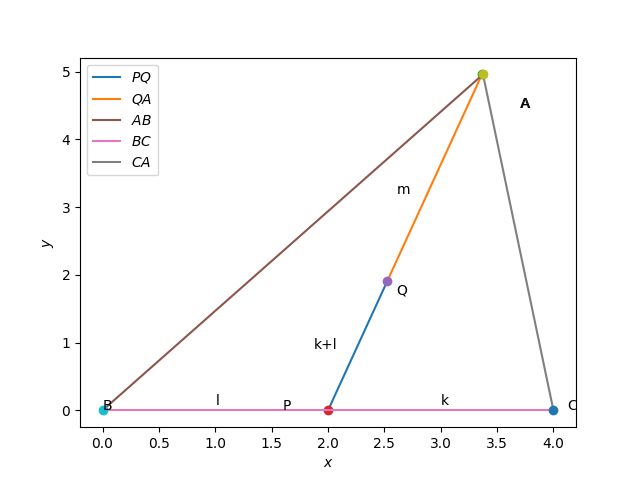
\includegraphics[width =\linewidth]{Figure_1.png}
        \caption{Triangle ABC with vertices A(3.366,4.96), B(0,0), C(4,0), and P(2,0), Q(2.5,1.98) are used for python plot.}\label{t1}
\end{figure}
Consider Fig.\ref{t1}
\begin{align}
    \vec{B}=\myvec{x_1\\y_1},
    \vec{C}=\myvec{x_2\\y_2},
     \vec{A}=\myvec{x_3\\y_3}
\end{align}
The line joining  $\vec{BC}$ divided into the ratio l:k at point of division $\vec{P}$ can be written as
\begin{align}
    l\brak{\vec{CP}}=k\brak{\vec{PB}}
\end{align}
\begin{align}
    l\brak{\vec{P-C}}=k\brak{\vec{B-P}}
\end{align}
\begin{align}
    \brak{l+k}\vec{P}=l\vec{C}+k\vec{B}
\end{align}
\begin{align}
    \brak{l+k}\vec{P}=\myvec{\vec{C} & \vec{B}}\myvec{l\\k}
\end{align}
\begin{align}
     \vec{P}=\frac{1}{l+k}\myvec{x_2&x_1\\y_2&y_1}\myvec{l\\k}
\end{align}
\begin{align}
     \vec{P}=\frac{1}{l+k}\myvec{x_2l+x_1k\\y_2l+y_1k}
\end{align}
\begin{align}
     \vec{P}=\myvec{\frac{x_2l+x_1k}{l+k}\\\frac{y_2l+y_1k}{l+k}}
\end{align}
Now,the line joining $\vec{PA}$ divided into the ratio m:k+l at point of division $\vec{Q}$ can be written as
\begin{align}
    \brak{l+k}\brak{\vec{PQ}}=m\brak{\vec{QA}}
\end{align}
\begin{align}
    \brak{l+k}\brak{\vec{Q-P}}=m\brak{\vec{A-Q}}
\end{align}
\begin{align}
    \brak{l+k+m}\vec{Q}=m\vec{A}+\brak{l+k}\vec{P}
\end{align}
\begin{align}
    \brak{l+k+m}\vec{Q}=\myvec{\vec{A} & \vec{P}}\myvec{m\\l+k}
\end{align}
\begin{align}
    \vec{Q}=\frac{1}{l+k+m}\myvec{x_3&\frac{x_2l+x_1k}{l+k}\\y_3&\frac{y_2l+y_1k}{l+k}}\myvec{m\\k+l}
\end{align}
\begin{align}
    \vec{Q}=\frac{1}{l+k+m}\myvec{mx_3+\brak{k+l}\frac{x_2l+x_1k}{l+k}\\my_3+\brak{k+l}\frac{y_2l+y_1k}{l+k}}
\end{align}
\begin{align}
    \vec{Q}=\frac{1}{l+k+m}\myvec{mx_3+x_2l+x_1k\\my_3+y_2l+y_1k}
\end{align}
\begin{align}
    \vec{Q}=\myvec{\frac{mx_3+x_2l+x_1k}{l+k+m}\\\frac{my_3+y_2l+y_1k}{l+k+m}}
\end{align}
Hence, Q is the required coordinate of the latter point of section.
\end{document}

